% 10/06/2017 
%LaTex version of my CV

\documentclass[10pt,a4paper]{article}
\usepackage[left=0.7in, top=0.65in, right=0.7in, bottom=0.6in]{geometry}
\usepackage{enumerate} % put in numbers or bullet points
\usepackage{setspace}	% line spacing					
\usepackage{eurosym}
\usepackage{graphicx,lipsum}
\usepackage{wrapfig}

%\usepackage{fullpage}
\usepackage{fancyhdr}
\pagestyle{fancy} % page numbers and headers and footers

\usepackage{lipsum}

\newcommand\textbox[1]{%
  \parbox{.333\textwidth}{#1}%
}


\usepackage{amsmath}

\newcommand{\textoperatorname}[1]{%
  \operatorname{\textnormal{#1}}%
}


 

\fancyhead[RO,RE]{Dr Kevin Healy CV}
\fancyfoot[C]{\thepage~of 8}

\renewcommand{\headrulewidth}{0.1pt}
\renewcommand{\footrulewidth}{0pt}

\renewcommand*{\familydefault}{\sfdefault} %% I changed the font
\usepackage{helvet}

%\usepackage[osf]{mathpazo} % palatino font package
%\usepackage{fontspec} %this must be in XeLaTeX
%\setmainfont{Verdana}%
%\setmainfont{Calibri}%
%\setsansfont{Tahoma}%
%\setmainfont{Helvetica}%
%\setmainfont{Garamond}%
\usepackage{hyperref} % allows the inclusion of hyperlinks




\usepackage{titlesec} % Used to customize the \section command
\titleformat{\section}{\Large\raggedright}{}{0em}{} [\titlerule] % Text formatting of sections
\titlespacing{\section}{0pt}{3pt}{10pt} % Spacing around sections (left, above, below)

\begin{document}

\par{\centering{\Huge \textbf{Dr Kevin {Healy}}}\smallskip\par}

\smallskip

\large\centering{Lecturer in Zoology (Below the Bar)\\ 
National University of Ireland, Galway,\\
Martin Ryan Institute,\\
Galway, Ireland}\\
\bigskip
\bigskip


\noindent\textbox{kevin.healy@nuigalway.ie}\textbox{\hfil \href{http://scholar.google.com/citations?user=5Kb9u8EAAAAJ}{Google Scholar} \hfil}\textbox{\hfill \href{https://www.nuigalway.ie/zoology/research/macroecology/}{NUIG website page}}

\bigskip
\bigskip

\section{\textbf{Career Overview}}

Since joining NUI Galway in 2019 I have published my macroecology research in high ranking journals, won research funding, built international and cross school collaborations and in 2021 I was awarded the Irish Ecological Associations early career researcher award.\\
\smallskip
\smallskip


I deliver teaching for eight modules (20.44 student FTE) where I incorporate cutting edge pedagogic methods, which I developed through completing a Certificate in Higher Education, and I have supervised 2 Phd students (1 graduated) and co-supervise 2 masters students.\\
\smallskip
\smallskip


I have also contributed to the School and Community through initiating the Galway Ecology and Evolution Group, contributing to committees and representing NUI Galway on an international stage through engaging with media, such as the BBC, Netflix and the Irish Times.

\bigskip
\bigskip

\section{\textbf{Academic Career}}

\raggedright	
\textbf{2019 - Present:} Lecturer (Below the Bar), The National University of Ireland, Galway.\\ 
Made permanent in post 1\textsuperscript{st} January 2020.
\bigskip

\raggedright	
\textbf{2017 - 2018:} Marie Sk\l{}odowska-Curie Individual Fellow, The University of St Andrews.
\par{\fontsize{10.5}{10} Funded by the European Commission Horizon 2020 program.\bigskip} 

\raggedright	
\textbf{2015 - 2017:} Post Doctoral research position in Zoology, Trinity College Dublin.
 \smallskip
\par{\fontsize{10.5}{10} Prof Yvonne Buckley's research group. Funded by Science Foundation Ireland.\bigskip} 

\smallskip
\smallskip


\section{\textbf{Education}}

\raggedright	
\textbf{2011 - 2015:} Ph.D. in Zoology, Trinity College Dublin. Supervised by Dr Andrew Jackson.\\ 
Funded through the Earth and Natural Sciences Doctoral Studies Programme.

\bigskip

\textbf{2007-2011:} B.A. Mod in Zoology, First class honours (77\%), Trinity College Dublin.\\

\bigskip


\section{\textbf{Awards}}

\raggedright	

\textbf{2021:} Early Career Achievement Award, presented by the Irish Ecological Association.\\
\smallskip
\smallskip


\textbf{2017:} Innovations in Sustainability Award from the Ecological Society of America based on\\ 
\hspace{11 mm} the publication Donohue \textit{et al} 2017.

\smallskip

\textbf{2017:} Early Career Award and Plenary talk for the British Ecology Society Macroecology\\  
\hspace{11 mm} Special Interest group.\\ 

\textbf{2011:} Awarded the Gold medal for "exceptional degree merit" in my B.A Mod. Zoology.\\ 

\clearpage







\section{\textbf{Research and Scholarly Standing}}



My research is in the field of macroecology where I address fundamental questions on topics relating to population dynamics, trophic ecology and theoretical ecology.\\ 
\smallskip
\smallskip

\begin{wrapfigure}{r}{2in}
\flushright
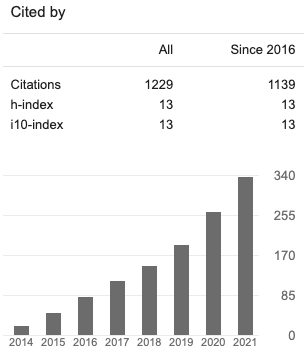
\includegraphics[width=2in]{google_scholar_2021.jpg}
%\caption{Google Scholar citation 17/11/2021.}
\end{wrapfigure}

Since joining NUI Galway I have published papers in top\\ journals including \textit{Nature Ecology and Evolution}, and\\ \textit{Nature Communications}, I have increased my h-index\\ from 6 to 13, my i10-index from 5 to 13 and the total\\ number of citations for my research from 401 to 1236.
\smallskip
\smallskip

I have successfully acquired research funding, including\\ an IRC COALESCE and an IRC postgraduate award and\\ increased my international research standing through\\ invited presentations and keynote talks, being invited to\\ be editor of a special issue for \textit{Toxins} and developing\\ my international collaboration network.\\
\smallskip
\smallskip
Based on my contribution to the field of Ecology I was\\ 
awarded the 2021 Early Career Achievement Award\\ 
by the Irish Ecological Association.\\

\bigskip
\bigskip



%	Awards and Grants
%----------------------------------------------------------------------------------------


\section{\textbf{Funding awards}}
\par
Since, joining NUI Galway I have applied for 7 funding calls and have won over \euro 500,000 in funding awards for research activities in my career to date. I have two funding applications currently under review, and an ERC Starting grant currently under submission. 


\bigskip

\textit{Successful awards}
\smallskip
\smallskip

\begin{tabular}{ll}
\textbf{2021:} & IRC COALESCE Award in collaboration with Dr David Doyle in Maynooth\\
& University (\euro 190,803.30).\\
\textbf{2020:} & British Ecology Society funds for a coding workshop I ran in NUI Galway (\euro 1200).\\
\textbf{2019:} & IRC Postgraduate award for current PhD student Keith Lyons (\euro 80,000).\\
\textbf{2017:} & Marie Sk\l{}odowska-Curie Individual Fellowship (MSCA-IF). Funded by Horizon\\
& 2020 (\euro 183,454.80).\\
\textbf{2017:} & Government of Ireland Postdoctoral Fellowship. Funded by the Irish Research\\
& Council (\euro 91,330) *I declined this award to accept the MSCA-IF.\\
\textbf{2014:} & Gordon Research Seminar mentoring program position. Funded by Gordon\\
& Research Conferences and the National Science Foundation. (\euro 1,300)\\
\end{tabular}

\smallskip

\textit{Funding awards under review/submission}
\smallskip

\begin{tabular}{ll}
\textbf{2022:} & ERC Starting Grant (Currently under submission).\\
\textbf{2021:} & North-South Research Programme SFI with Dr Daniel Pincheira-Donoso\\ 
& (Queens University Belfast) (Currently under review \euro 156,717.50).\\
\textbf{2021:} & IRC Postgraduate award (Currently under review \euro 80,000).\\
\end{tabular}
\smallskip

\textit{Unsuccessful awards}
\smallskip
\smallskip

\begin{tabular}{ll}
\textbf{2020:} & EMFASIS: Horizon 2020 H2020-BG call: Multi-partner call on Blue growth.\\
& Made final evaluation stage (NUIG portion of award \euro 345,282.29).\\
\textbf{2020:} & Welcome Trust: Snakebite Grants: Discovering and Developing New Treatments\\
 & Rejected during review (\euro 500,000).\\
\textbf{2019:} & IRC Postgraduate award (Rejected during review \euro 80,000).\\
\end{tabular}


\bigskip


\pagebreak


%-------------------------------------
% Publications
%--------------------------------------
\section{\textbf{Publications}}
\begin{flushleft}

I have published 15 peer review publications to date, 7 of which I have published since joining NUI Galway in 2019. My publications have been cited a total of 1236 times, my h-index is 13 and my i10-index is 13 (\href{http://scholar.google.com/citations?user=5Kb9u8EAAAAJ}{Google Scholar}). All citations below are from Google scholar. JIF = Journal Impact Factor. 


\begin{normalsize}

{\center \large \textbf{2021} \par}

\smallskip

\hspace{10 mm} \setlength{\parindent}{0mm} Kelly, R., \textbf{Healy, K.,} Anand, M., Baudraz, M.E.A., Bahn, M., Cerabolini, B.E.L., Cornelissen, J.H.C., Dwyer, J.M., Jackson, A.L., Kattge, J., Niinemets, U., Penuelas, J., Pierce, S., Salguero-G\'{o}mez, R., Buckley, Y.M. 2021. Climatic and evolutionary contexts are required to infer plant life history strategies from functional traits at a global scale \textit{\textbf{Ecology Letters}},  24, 970-983. \href{https://onlinelibrary.wiley.com/doi/full/10.1111/ele.13704}{ Link to paper}. JIF = 9.492. 4 citations.

{\center \large \textbf{2020} \par}

\smallskip

\hspace{10 mm} \setlength{\parindent}{0mm} Guillerme, T., Cooper, N., Brusatte, S.L., Davis, K.E., Jackson, A.L., Gerber, S., Goswami, A., \textbf{Healy, K.,} Hopkins, M.J., Jones, M.E.H., Lloyd, G.T., O'Reilly, J.E., Pate, A., Puttick, M.N., Rayfield, E.J., Saupe, E.E., Sherratt, E., Slater, G.J., Weisbecker, V., Thomas, G.H., Donoghue, P.C.J. 2020. Disparities in the analysis of morphological disparity. \textit{\textbf{Biology Letters}},  16, 20200199. \href{https://royalsocietypublishing.org/doi/full/10.1098/rsbl.2020.0199}{Link to paper}. JIF = 3.703. 14 citations.

\smallskip
\smallskip

\hspace{10 mm} \setlength{\parindent}{0mm}  Mooney, A., Conde, A.D., \textbf{Healy, K.,} and Buckley, Y.M. 2020. A system wide approach to managing zoo collections for visitor attendance and in situ conservation. \textit{\textbf{Nature Communications}}, 11, 1-8. \href{https://www.nature.com/articles/s41467-020-14303-2}{Link to paper}. JIF = 15.805. 8 citations.

\smallskip
\smallskip

\hspace{10 mm} \setlength{\parindent}{0mm}  Lyons, K., Dugon, M.M., \textbf{Healy, K.} 2020. Diet Breadth Mediates the Prey Specificity of Venom Potency in Snakes. \textit{\textbf{Toxins}},  12, 74. \href{https://www.mdpi.com/2072-6651/12/2/74}{Link to paper}. JIF = 3.531, 26 citations.


{\center \large \textbf{2019} \par}

\smallskip

\hspace{10 mm} \setlength{\parindent}{0mm}\textbf{Healy, K.,} Ezard, T.H.G., and Jones, O.R., Salguero-G\'{o}mez, R., and Buckley, Y.M. 2019. Animal life history is shaped by the pace of life and the distribution of age-specific mortality and reproduction. \textit{\textbf{Nature Ecology and Evolution}},  3, 1217-1224. \href{https://www.nature.com/articles/s41559-019-0938-7}{Link to paper}. JIF = 15.46, 78 citations.

\smallskip
\smallskip

\hspace{10 mm} \setlength{\parindent}{0mm}\textbf{Healy, K.,} Carbone, C., and Jackson, A.L. 2019. Snake venom potency and yield are associated with prey evolution, predator metabolism and habitat structure. \textit{\textbf{Ecology Letters}}, 22, 527-537. \href{https://onlinelibrary.wiley.com/doi/abs/10.1111/ele.13216}{Link to paper}. JIF = 9.492, 31 citations.

{\center \large \textbf{2017} \par}

\smallskip

\hspace{10 mm} \setlength{\parindent}{0mm}\textbf{Healy, K.,} Guillerme, T., Kelly, S.B.A., Inger, R., Bearhop, S., Jackson, A.L. 2017. SIDER: an R package for predicting trophic discrimination factors of consumers based on their ecology and phylogenetic relatedness. \textit{\textbf{Ecography}}. \href{https://onlinelibrary.wiley.com/doi/abs/10.1111/ecog.03371}{Link to paper}. JIF = 6.45, 69 citations.

\smallskip
\smallskip

\hspace{10 mm} \setlength{\parindent}{0mm} Adam Kane, \textbf{Healy, K.,}, Guillerme, T., Ruxton, G., and Jackson A.L. 2017. A recipe for scavenging and natural history. \textit{\textbf{Ecography}}. \href{https://onlinelibrary.wiley.com/doi/pdf/10.1111/ecog.02817}{Link to paper}. JIF = 6.45, 27 citations.


{\center \large \textbf{2016} \par}

\smallskip

\hspace{10 mm} \setlength{\parindent}{0mm}Kane, A., \textbf{*Healy, K.,} Ruxton, G.D., and Jackson, A.L. 2016. Body size drives importance of scavenging in theropods. \textit{\textbf{The American Naturalist}}. \textbf{6} (187), 706-716. \href{https://www.researchgate.net/profile/Kevin_Healy/publication/301279301_Body_Size_as_a_Driver_of_Scavenging_in_Theropod_Dinosaurs/links/570f8b2a08ae38897ba19c35.pdf.}{Link to paper}. *Joint-First author. JIF = 4.265, 17 citations.

\smallskip
\smallskip

\hspace{10 mm} \setlength{\parindent}{0mm}Donohue, I., Hillebrand, H., Montoya, J.M., Petchey, O.L., Pimm, S.L., Fowler, M.S., \textbf{Healy, K.,} Jackson, A.L., Lurgi, M., McClean, D., O'Connor, N.E., O'Gorman, E.J., Yang, Q. 2016. Navigating the complexity of ecological stability. \textit{\textbf{Ecology Letters}}. 19 (9), 1172-1185. \href{https://onlinelibrary.wiley.com/doi/abs/10.1111/ele.12648}{Link to paper}. JIF = 9.492, 316 JIFcitations.

{\center \large \textbf{2014} \par}

\smallskip

\hspace{10 mm} \textbf{Healy, K}., Guillerme, T., Finlay, S., Kane, A., Kelly, S.B.A., McClean, D., Kelly, D.J., Donohue, I., Jackson, A.L. and Cooper, N., 2014. Ecology and mode-of-life explain lifespan variation in birds and mammals. \textit{\textbf{Proceedings of the Royal Society B}}, \textbf{281}(1784), 20140298. \href{http://rspb.royalsocietypublishing.org/content/281/1784/20140298}{Link to paper}. JIF = 5.349, 189 JIF citations.


{\center \large \textbf{2013} \par}

\smallskip

\hspace{10 mm} \textbf{Healy, K}., McNally, L, Ruxton, G., Cooper, N. and Jackson, A.L. 2013. Metabolic rate and\\
body size linked with perception of temporal information.  \textit{\textbf{Animal Behaviour}}. \textbf{86}, 685-696. \href{http://dx.doi.org/10.1016/j.anbehav.2013.06.018}{Link to paper}. JIF = 2.689, 147 citations. 

\smallskip
\smallskip


\hspace{10 mm} \setlength{\parindent}{0mm}Donohue, I., Petchey, O.L., Montoya, J.M., Jackson, A.L., McNally, L., Viana, M., \textbf{Healy, K}., Lurgi, M., O’Connor, N.E. and Emmerson, M.C. 2013. On the dimensionality of ecological stability. \textit{\textbf{Ecology Letters}}. \textbf{16}, 421-429. \href{http://onlinelibrary.wiley.com/doi/10.1111/ele.12086/abstract} {Link to paper}. JIF = 9.492, 262 citations.
\bigskip


\textbf{\textit{Comment response}}\\
\hspace{10 mm} \setlength{\parindent}{0mm}\textbf{Healy, K}. 2015.  Eusociality but not fossoriality drives longevity in small mammals. \textit{\textit{Proceedings of the Royal Society B}}, \textbf{282}, 20142917. \href{http://rspb.royalsocietypublishing.org/content/282/1806/20142917} {Link to paper}. JIF = 5.349, 14 citations.

\bigskip

\textbf{\textit{Statistical packages}}\\
\hspace{10 mm} \setlength{\parindent}{0mm} Guillerme, T., \textbf{Healy, K.,} 2014. mulTree: a package for running MCMCglmm analysis on multiple trees. ZENODO. DOI: 10.5281/zenodo.12902. 29 citation.

\bigskip

\textbf{\textit{Book chapters}}\\
\hspace{10 mm} \setlength{\parindent}{0mm} Jones, O., Ezard, T., Dooley, C., \textbf{Healy, K.,}  Hodgson, D.J., Mueller, M., Townley, S., Salguero-Gomez, R. 2019. My family and other animals: human demography under a comparative cross-species lens: comparative human demography. In, Sear, Rebecca and Burger, Oskar (eds.) Human Evolutionary Demography. 3 citations.
\bigskip

\end{normalsize}


\section{Ongoing collaboration groups}


\textbf{Venom evolution collaboration} with Dr Michel Dugon (NUI Galway) and Prof. Nicholas\\ 
Casewel (Liverpool School of Tropical Medicine). Previously submitted funding application\\
to the Welcome Trust and also inputting to my ERC Starting Grant submission.\\

\smallskip
\smallskip

\textbf{De-extinciton collaboration} with Dr David Doyle (Maynooth University). Currently funded\\
 by an IRC COALESCE funding grant.\\

\smallskip
\smallskip

\textbf{Biogeography of extinction collaboration} with Dr Daniel Pincheira-Donoso of (Queens\\
University Belfast). Application submitted to SFI North-South Research Programme.\\ 

\smallskip
\smallskip


\textbf{Stable Isotopes working group}. Collaborative research group I lead, including Dr Chris Harrod (Universidad de Antofagasta), Prof Stuart Bearhop (University of Exeter), Prof Edwin Niklitschek (Universidad de Los Lagos) and Dr Andrew Jackson (Trinity College Dublin) developing and updating the SIDER statistical package (\href{https://github.com/healyke/SIDER}{Link to package}).\\

\smallskip
\smallskip


%---------------------------------------
\textbf{Timespines working group}. Collaborative group, including Dr Adam Kane (UCD), Dr Thomas Guillerme (University of Sheffield) and Prof Lauren Sallan (University of Pennsylvania), using paleontological data to test drivers of the evolution of defensive structures in animals.\\ 

\smallskip
\smallskip

%---------------------------------------
\textbf{African Biogeography collaborative} led by Prof. Ara Monadjem (University of Swaziland).\\
Paper currently under review at \textit{Global Ecology and Biogeography.}\\

\smallskip
\smallskip

\textbf{Island Biogeogrpahy working group}. Collaborative group including Dr Anna Csergo (Szent Istv�n University), Yvonne Buckley (TCD) and Ruth Kelly (Agri-Food and Biosciences Institute, Belfast) using big data to test drivers of island evolution. Two publications under submission.\\

\smallskip
\smallskip

\textbf{Life History working group}. Collaboration including Prof Michael Kearney (The University of Melbourne), Yvonne Buckley (TCD), Ruth Kelly (Agri-Food and Biosciences Institute, Belfast) and Dr Angela Carnevale (NUI Galway), developing tools and testing macroecology theory of life history. One publication currently under submission.\\
\bigskip

\center
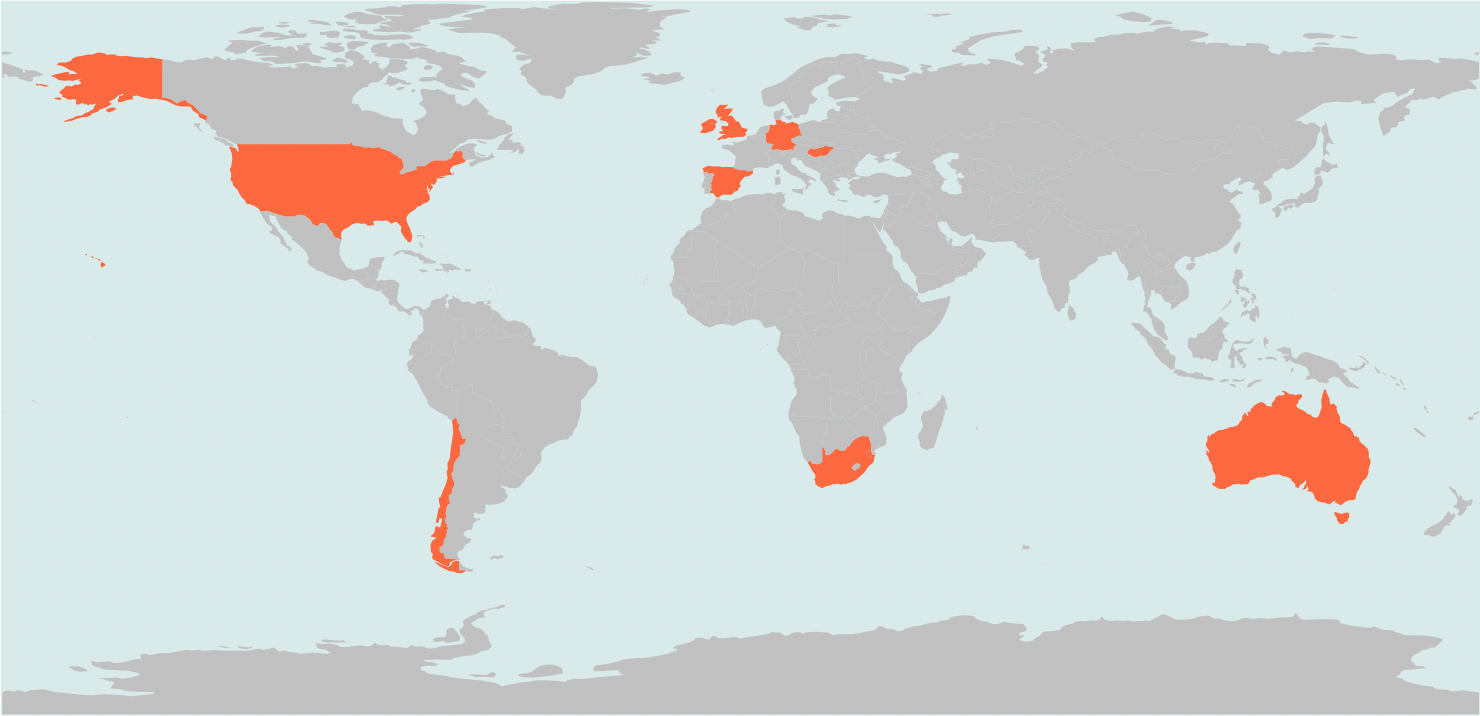
\includegraphics[width=5in]{Col_map.png}
\\
Map of Collaborations
\\

%--------------------------



\clearpage
\section{\textbf{Learning, Teaching and Assessment}}
\raggedright{I am involved in delivering eight modules, teaching 20.44 student FTEs and I am the coordinator for three modules and the 2nd year Zoology coordinator. I currently supervise one PhD student, co-supervise two Masters students projects and I have co-supervised a PhD student who graduated in 2020. I continually develop my teaching through engaging with CELT and have completed a Postgraduate Certificate in Higher Education.}


{\center \textbf{Undergraduate Teaching}\par}

{\center \textit{2nd Year} \par}

\textbf{2nd year Zoology coordinator} This role involved coordinating the transition to online teaching and assessments, including managing exams and taking the lead on detecting and following up on plagiarism cases. It also includes running advisory sessions and assisting students throughout the year.

\smallskip
\smallskip

\begin{tabular}{ll}
\textbullet& \textbf{ZO208}: Invertebrate Zoology (\textit{5 ECTS}). Class of approximately 150 students,\\
& 12 lecture hours, four practical sessions (FTE = 8.33).This module received extremely\\ 
& positive reviews in an independent teaching review in 2021, with particularly positive\\ 
& feedback on the use of H5P online workbooks.\\ 
& \textbf{Module coordinator:} Coordination of this module has included scheduling practical\\ 
& sessions, compiling exam papers for the external examiner and managing the online\\ 
& transition of teaching in 2020 and 2021.\vspace{2mm} 
\\
\textbullet& \textbf{ZO209}: Vertebrate Zoology (\textit{5 ECTS}). Class of approximately 150 students, 6 lecture\\
&hours, two practical sessions (FTE = 4.16). As in ZO208 I use a combination of H5P\\
& workbooks, online and in class lectures to aid in teaching.\\ 
& \textbf{Module coordinator:} Coordination of this module has included scheduling practical\\ 
& sessions, compiling exam papers for the external examiner and managing the online\\ 
& transition of teaching in 2020 and 2021.\\
\end{tabular}

{\center \textit{3rd Year} \par}

\begin{tabular}{ll}

\textbullet& \textbf{ZO320}: Concepts in Population and Community Ecology (\textit{5 ECTS}). Class of\\ 
& approximately 90 students, 6 lecture hours, two practical sessions (FTE = 2.5).\\
& Peer review of this teaching, as part of CEL262, and student questioner feedback\\ 
& positively highlighted my use of online simulations tools for teaching and assessment\\ 
& and the use of H5P online workbooks.\\
\end{tabular}

{\center \textit{4th Year} \par}

\begin{tabular}{ll}

\textbullet& \textbf{ZO417}: Marine and Coastal Ecology(\textit{5 ECTS}). Class of approximately 50 students,\\ 
&12 lecture hours (FTE = 2.5). I implemented a flipped classroom approach using apps,\\
&podcasts and publications. Questioners gave positive feedback for this approach.\vspace{2mm} 
\\

\textbullet& \textbf{ZO4101} and \textbf{MR413}: Zoology and Marine Research projects (\textit{20 ECTS}). I have\\ 
& supervised 10 research projects since 2020 (with three ongoing, FTE = 1.3), five have\\
& achieved firsts, one won best Zoology project and two are undergoing publication.\vspace{2mm} 
\\

\textbullet& \textbf{ZO425}: Litrature Review (\textit{10 ECTS}). Supervision of two reviews each year (FTE =1.3).\vspace{2mm} 
\\

\textbullet& \textbf{ZO409}: Marine Science Essay and Presentation (\textit{5 ECTS}). Supervision of two reviews\\ 
& each year (FTE = 0.17).\vspace{2mm} 
\\

\textbullet& \textbf{ZO416}: Integrative Zoology (\textit{5 ECTS}). Class of approximately 35. I run a two hour\\ 
& flipped classroom with an essay assessment (FTE = 0.47).\\ 
& \textbf{Module coordinator:} Coordination in this role includes managing the schedule of\\ 
& lecturer contributions and communication with students.\vspace{2mm} 
\\

\textbullet& \textbf{ZO414}: Advanced Zoology Topics (\textit{5 ECTS}). Class of approximately 35. I set and\\ 
& assess 1/6 of the reading material covered in this self directed module (FTE = 0.23). \vspace{2mm} 
\\

\end{tabular}

\clearpage

\raggedright\textbf{Post Graduate Teaching}\\
\begin{tabular}{ll}
\textbullet&  I am currently supervisor for one PhD student in NUI Galway and as co-supervisor\\
& oversaw the graduation of one student based in Trinity College Dublin.\\
\textbullet&  I am currently co-supervising two masters student projects with Dr Michel Dugon\\
\textbullet& I won funding for and ran a two day international statistics workshop in NUI Galway\\ 
& in 2020 for 35 attendees. Funded by the British Ecology Society (\euro 1200).\\
\end{tabular}

\bigskip

\raggedright\textbf{Professional Training}\\
\begin{tabular}{ll}
\textbf{2021:} & I am currently completing the Learning Technologies (CEL263) module run by\\
& the Centre for Excellence in Learning and Teaching (5 ECTS).\\
\textbf{2021:} & I completed the Postgraduate Certificate in Higher Education delivered by the\\
& Centre for Excellence in Learning and Teaching (30 ECTS).\\
\textbf{2020:} & I completed the Teaching Online module (CEL263) delivered by the Centre for\\
& Excellence in Learning and Teaching (5 ECTS).\\
%------------------
\textbf{2019:} & I completed a workshop on research student supervision run by Prof Lucy\\ 
& Byrnes, NUI Galway.\\

\textbf{2019:} & I completed a workshop on T4 Site Managing, NUI Galway.\\
%------------------
\end{tabular}

\bigskip
\bigskip

\section{\textbf{Contribution to School, University and Community}}
My contributions to the School, University, and Community include committee roles; reviewing dissertations, research and grants; building more open and engaged academic communities and promoting the university through open days, conferences and the media.
\smallskip
\smallskip

\raggedright\textbf{School committees contributions}\\
\begin{tabular}{ll}
\textbullet& I have represented the Zoology Department on the School, Education and Students\\
& Committee since 2019. My contributions on this committee includes proposing changes\\ 
& to Zoology teaching and implementing agreed changes on the Akari system; providing\\ 
& feedback on proposed changes to modules and on assessment, such as plagiarism\\ 
& issues during COVID-19; and coordinating allocation of emergency funds to aid\\ 
& in the move to online teaching during COVID-19 lockdowns.\\
\textbullet& I have served on the Thomas Crawford Hayes Committee since 2019. My contributions\\
& include reviewing 10-20 funding applications each year and contributing to funding\\ 
& allocation decisions.\\
\textbullet& I have engaged with the School restructuring through the SNS Substructures and\\ 
& Business Plan working group, contributing to discussions and decisions relating to the\\ 
& new School's structure, name and how to develop engagement across the new School.\\
\end{tabular}

\smallskip
\smallskip

\raggedright\textbf{Graduate Examiner and committee contributions}\\
\smallskip

\begin{tabular}{ll}
\textbullet& \textbf{2021:} I was the internal examiner for the PhD examination of Dr Cesar Santana.\\ 
\textbullet& \textbf{2021:} I was the internal examiner for the PhD examination  of Dr Sophia Wassermann.\\ 
\textbullet& \textbf{2020:} I was chair of the PhD examinations committee for Dr Jasmine Headlam.\\ 
\textbullet& \textbf{2020:} I was the internal examiner for the PhD examination of Dr John Dunbar.\\ 
\textbullet& I currently sit on 12 School of Natural Science Graduate Research Committees.\\
& My contributions include reviewing graduate student progress annually and\\ 
& offering mentorship and support throughout the year.\\
\end{tabular}

\smallskip
\smallskip
\clearpage

\raggedright\textbf{External committees, editorial and evaluator boards}\\
\begin{tabular}{ll}
\textbullet& I have served on the BES Macroecology Special Interest Group committee since\\
& 2017. Current roles include organising a mentorship scheme and future meetings.\\
\textbullet& I was a committee member for the Irish Ecological Association from 2016 to 2018,\\
& and I was involved in developing the IEA Strategic Plan 2017-2021.\\ 
\textbullet& I am a currently the editor for a special issue for the journal \textit{Toxins} (\href{https://www.mdpi.com/journal/toxins/special_issues/venom_potency}{link to issue}).\\
\textbullet& I was an evaluator for the Marie Sk\l{}odowska-Curie Individual Fellowship 2021 call and\\
& a reviewer for German Research Federation and the Leverhulme Trust funding calls.\\
\textbullet& I have reviewed over 15 papers in the last 3 years for journals such as \textit{Nature Ecology}\\
&  \textit{and Evolution}, \textit{Nature Communications}, \textit{Ecology Letters}, \textit{Current Biology}, etc.\\
\end{tabular}

\smallskip
\smallskip

\raggedright\textbf{University Community contributions}\\
\begin{tabular}{ll}
\textbullet& I founded and run the Galway Ecology and Evolution group (GEEK club), which\\ 
& connects researchers across the School of Natural Sciences and provides opportunities\\ 
& to gain skills and provide a platform for researchers to engage\\
\textbullet& I am a member of the Biodiversity and Bioresources Research Cluster, where I engage\\
& with discussions regarding strategically targeting funding, providing feedback for,\\ 
& initiatives such as NUI Galway's Community and Sustainability Action Plan, and\\ 
& propose workshops such as through my GEEK group.\\
\textbullet& I am a member of the Open Scholarship Community Galway Group where I have\\
& engaged in open science workshops and invited founder, Hardy Schwamm, to discuss\\ 
& open science for a GEEK club session.\\
\textbullet& I have represented the Zoology Department and engaged with students\\ 
& for the last three Open days.\\
\textbullet& I run open R coding workshops available to undergraduates, postgraduates and\\ 
& staff across the School, with an uptake of approximately 15-25 this year.\\
\textbullet& I have contributed to developing an induction system for new staff as part of the\\ 
& SNS Athena Swan SAT process.\\
\textbullet& I have contributed to developing and maintaining the Zoology Department web page\\
& ilncuding taking a T4 web building course.

\end{tabular}

\smallskip

\raggedright\textbf{Outreach and Media}\\
\smallskip

\begin{tabular}{ll}
%---------------------------------------
\textbullet& I contributed towards research direction for Netflix series "Animal" aired 2021.\\
\textbullet& I was a guest on the award winning NPR Invisibilia podcast series aired 2021.\\
\textbullet& I discussed my research on the BBC podcast "A Sense of Time" (\href{https://www.bbc.co.uk/programmes/m0003qxf}{link to podcast}).\\
\textbullet& I wrote an RTE Brainstorm article on aging in animals published in 2020.(\href{https://www.rte.ie/brainstorm/2020/0203/1112818-why-do-some-animals-live-longer-than-others/}{link to article}).\\
\textbullet& My research featured in Scientific American in 2019 (\href{https://www.scientificamerican.com/podcast/episode/harder-working-snakes-pack-stronger-venom/
}{link to article}).\\
\textbullet& I featured on the RTE 2fm Dave Fanning Show in 2019 discussing my research.\\
\textbullet& My research was covered by the Irish Times print edition in 2019 and 2020.\\
\textbullet& Eight of my publications are in the top 98 percentile of altmetric scores.\\
\textbullet& I received two letters from NUI Galway President Ciar\'{a}n \'{O} h\'{O}gartaigh commending \\ 
& my role in increasing the standing of University in the wider community in relation to\\ 
& media coverage of my Venom research and separately my Time Perception research.\\

\end{tabular}

\smallskip
\smallskip

\raggedright\textbf{Invited talks and conferences}\\
\smallskip
\begin{tabular}{ll}
%-------------------------------
\textbf{2021:} & Keynote speaker for the European Evolution (EMPSEB XXVI) conference.\\
%-------------------------------
\textbf{2021:} & Invited seminar speaker to The University of Konstanz.\\
%-------------------------------
\textbf{2021:} & Presented at the Congress of the European Venom Network.\\
%-------------------------------
\textbf{2020:} & Invited seminar speaker to University College Dublin.\\
%-------------------------------
\textbf{2020:} & Presented at the British Ecological Association annual meeting.\\
%-------------------------------
\textbf{2018:} & Invited seminar speaker to Swansea University.\\
%-------------------------------
\textbf{2016:} & Invited seminar speaker to The University of Sheffield.\\
%-------------------------------
\end{tabular}
\smallskip
\smallskip

I have also presented at international conferences including the Ecological association of America (2017), Gordon Research Seminar (2014), ESEB XIV Congress
(2013 and 2019), EvoDemos (2016), IsoEcol (2012) and BES meetings (2013-2021).





\end{flushleft}

%-------------------------------------
% References
%--------------------------------------


\clearpage


\section{Internal References}

\begin{tabular}{cr}
\begin{minipage}[t]{3in}
\textbf{Dr\ Anne Marie Power}\\
Zoology Department\\
School of Natural Sciences\\
NUI Galway\\
Ireland\\
Tel: Ext. 3015\\
\href{mailto:annemarie.power@nuigalway.ie}{annemarie.power@nuigalway.ie}
\end{minipage}


&

\begin{minipage}[t]{2.2in}
\textbf{Prof\ XX}\\
Zoology Department\\
School of Natural Sciences\\
NUI Galway\\
Ireland\\
Tel: XXX\\
\href{mailto:X}{X}
\end{minipage}



\end{tabular}

\bigskip
\bigskip

\section{External References}

\begin{tabular}{lr}
\begin{minipage}[t]{3in}
\textbf{Dr\ Andrew L. Jackson}\\
Zoology Department\\
School of Natural Sciences\\
Trinity College Dublin\\
Dublin 2\\
Ireland\\
Tel: + 353 1 896 2728\\
\href{mailto:a.jackson@tcd.ie}{a.jackson@tcd.ie}
\end{minipage}


&

\begin{minipage}[t]{2.2in}
\textbf{Prof\ Yvonne Buckley}\\
Zoology Department\\
School of Natural Sciences\\
Trinity College Dublin\\
Dublin 2\\
Ireland\\
Tel: + 353 1 896 3172\\
\href{mailto:buckleyy@tcd.ie}{buckleyy@tcd.ie}
\end{minipage}




\end{tabular}



\end{document}